\begin{figure}
    \centering
    \footnotesize
    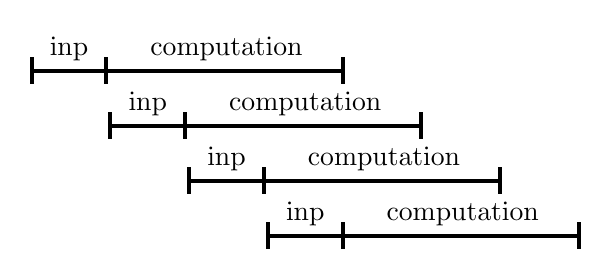
\begin{tikzpicture}
    \foreach \x in {0, 1, 2,...,3} {
        \draw[|-|, black, line width=0.5mm] (\x,-\x*0.7) to (\x+1,-\x*0.7);
        \path (\x,-\x*0.7) -- (\x+1,-\x*0.7) node [midway, above] {inp};
        \draw[-|, black, line width=0.5mm] (\x+1,-\x*0.7) to (\x+4,-\x*0.7);
        \path (\x+1,-\x*0.7) -- (\x+4,-\x*0.7) node [midway, above] {computation};
    }
    \end{tikzpicture}
    \caption{Parallelized beacon protocol, with offset input collection and overlapping computation.}\label{fig:beacon_parallel_timeline}
\end{figure}

